\normaltrue
\correctionfalse

%\UPSTIidClasse{11} % 11 sup, 12 spé
%\newcommand{\UPSTIidClasse}{12}

\exer{Roue motrice de chariot élévateur  $\star$ \label{A5:05:74}}
\setcounter{numques}{0}
\UPSTIcompetence[2]{A5-05}
\UPSTIcompetence[2]{A5-04}

\index{Compétence A5-05}
\index{Compétence A5-04}

\index{GPS}
\index{Spécification géométrique des produits}
\index{Roue motrice}

\ifcorrection
\else
\textbf{Pas de corrigé pour cet exercice.}
\fi

\ifprof
\else


On considère la roue motrice d'un chariot élévateur.

\begin{minipage}[c]{.5\linewidth}
\begin{center}
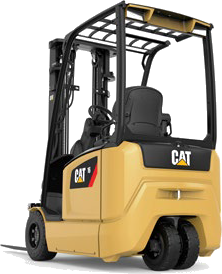
\includegraphics[height=5cm]{74_01}
\end{center}
\end{minipage} \hfill
\begin{minipage}[c]{.5\linewidth}
\begin{center}
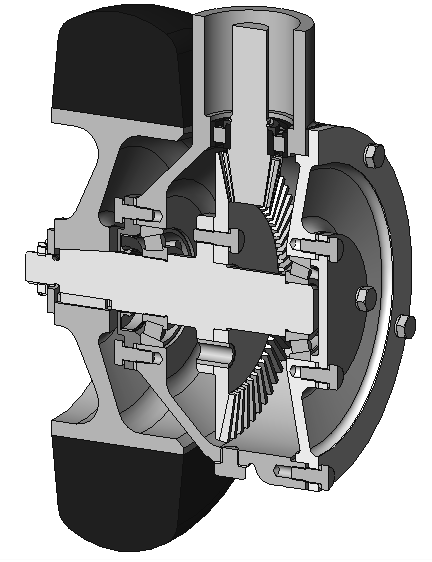
\includegraphics[height=5cm]{74_02}
\end{center}
\end{minipage} \hfill


\fi

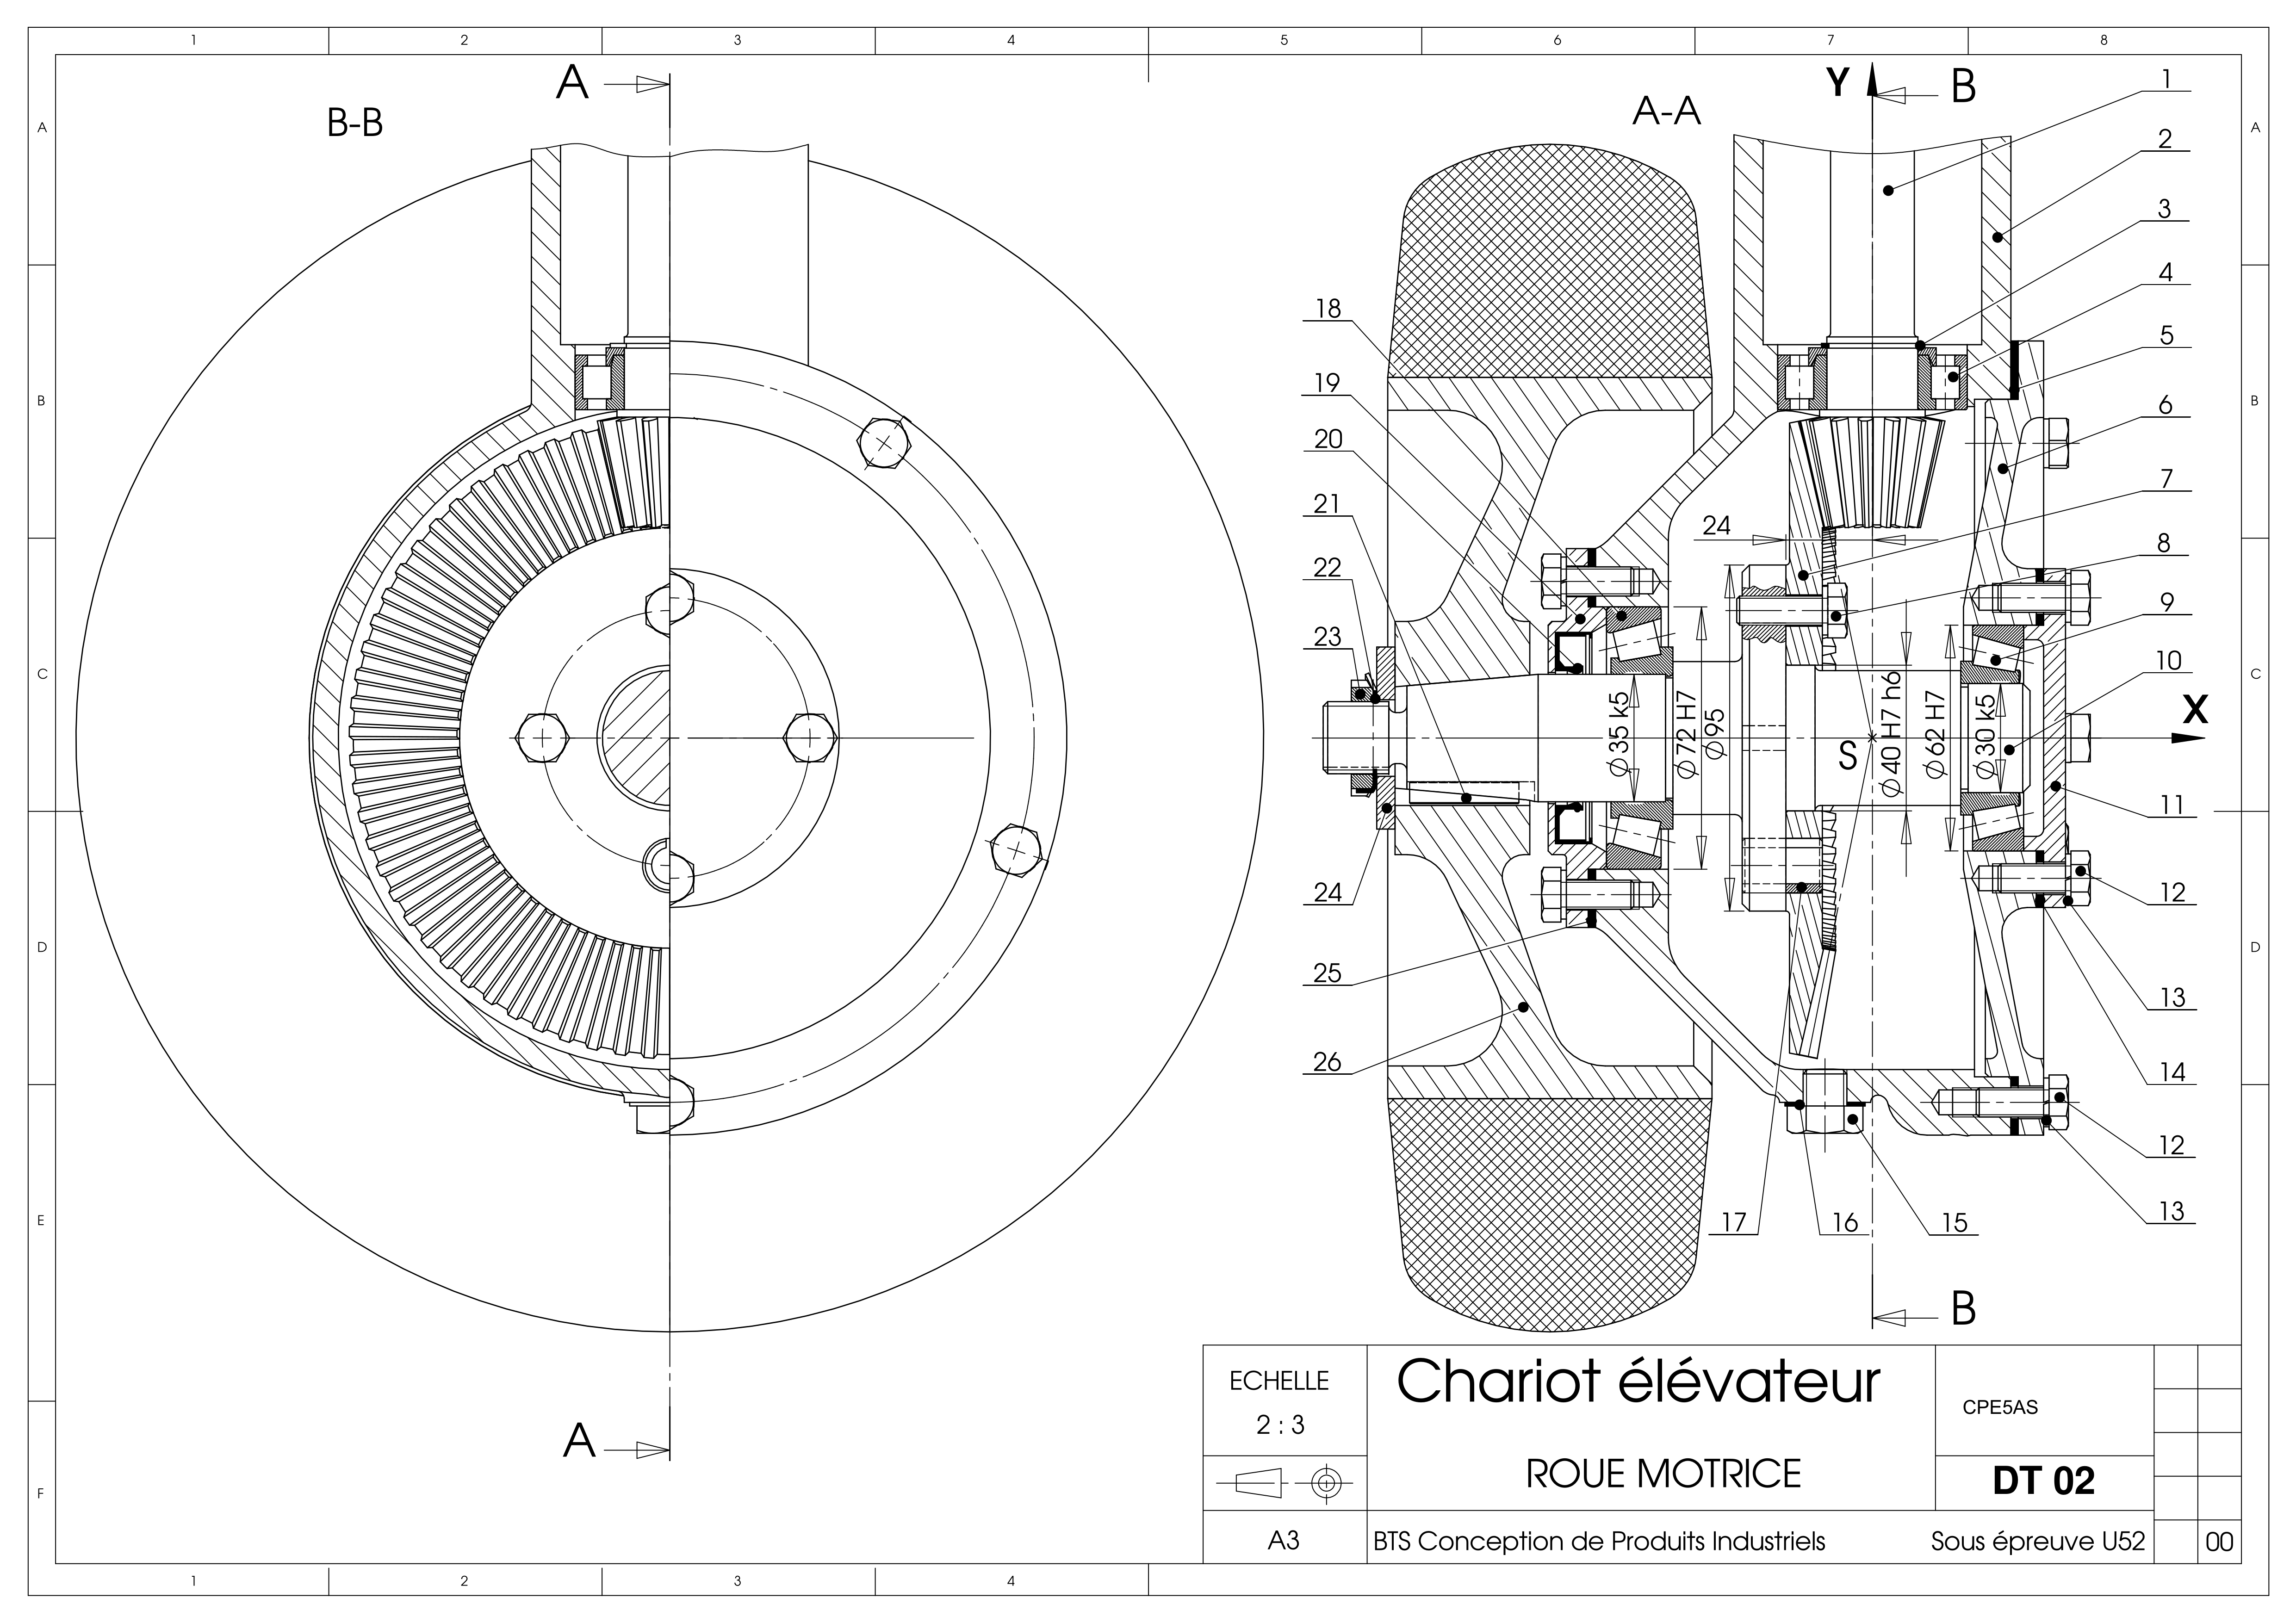
\includegraphics[width=\linewidth]{74_03}

\question{Justifier pourquoi les surfaces A, B et C ont été choisies comme éléments de référence ?}
\ifprof
\else
\fi

\question{Justifier pourquoi la surfaces F a été choisie comme élément de référence ?}
\ifprof
\else
\fi

\question{Décoder les spécifications suivantes : 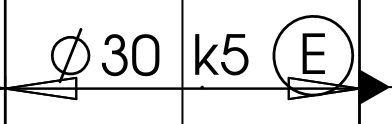
\includegraphics[height=0.8cm]{74_05} et 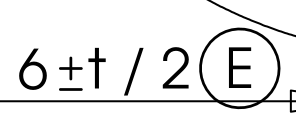
\includegraphics[height=0.8cm]{74_06}. Vous tracerez le gabarit associé à chacune des spécifications -- $30 k5 =30 ^{\begin{pmatrix}+2 \\ +18\end{pmatrix}}$.}
\ifprof
\else
\fi

\question{Décoder la spécification suivante 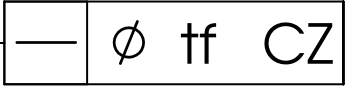
\includegraphics[height=0.8cm]{74_07}.}
\ifprof
\else
\fi

\question{Décoder la spécification suivante 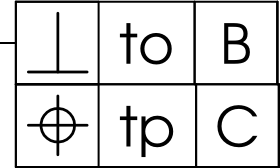
\includegraphics[height=1.2cm]{74_08}.}
\ifprof
\else
\fi

\question{Décoder la spécification suivante 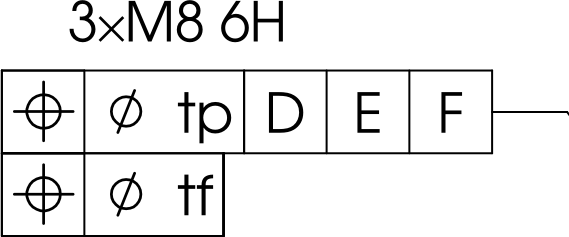
\includegraphics[height=1.5cm]{74_09}.}
\ifprof
\else
\fi

\question{Décoder la spécification suivante 
\includegraphics[height=0.8cm]{74_10}.}
\ifprof
\else
\fi



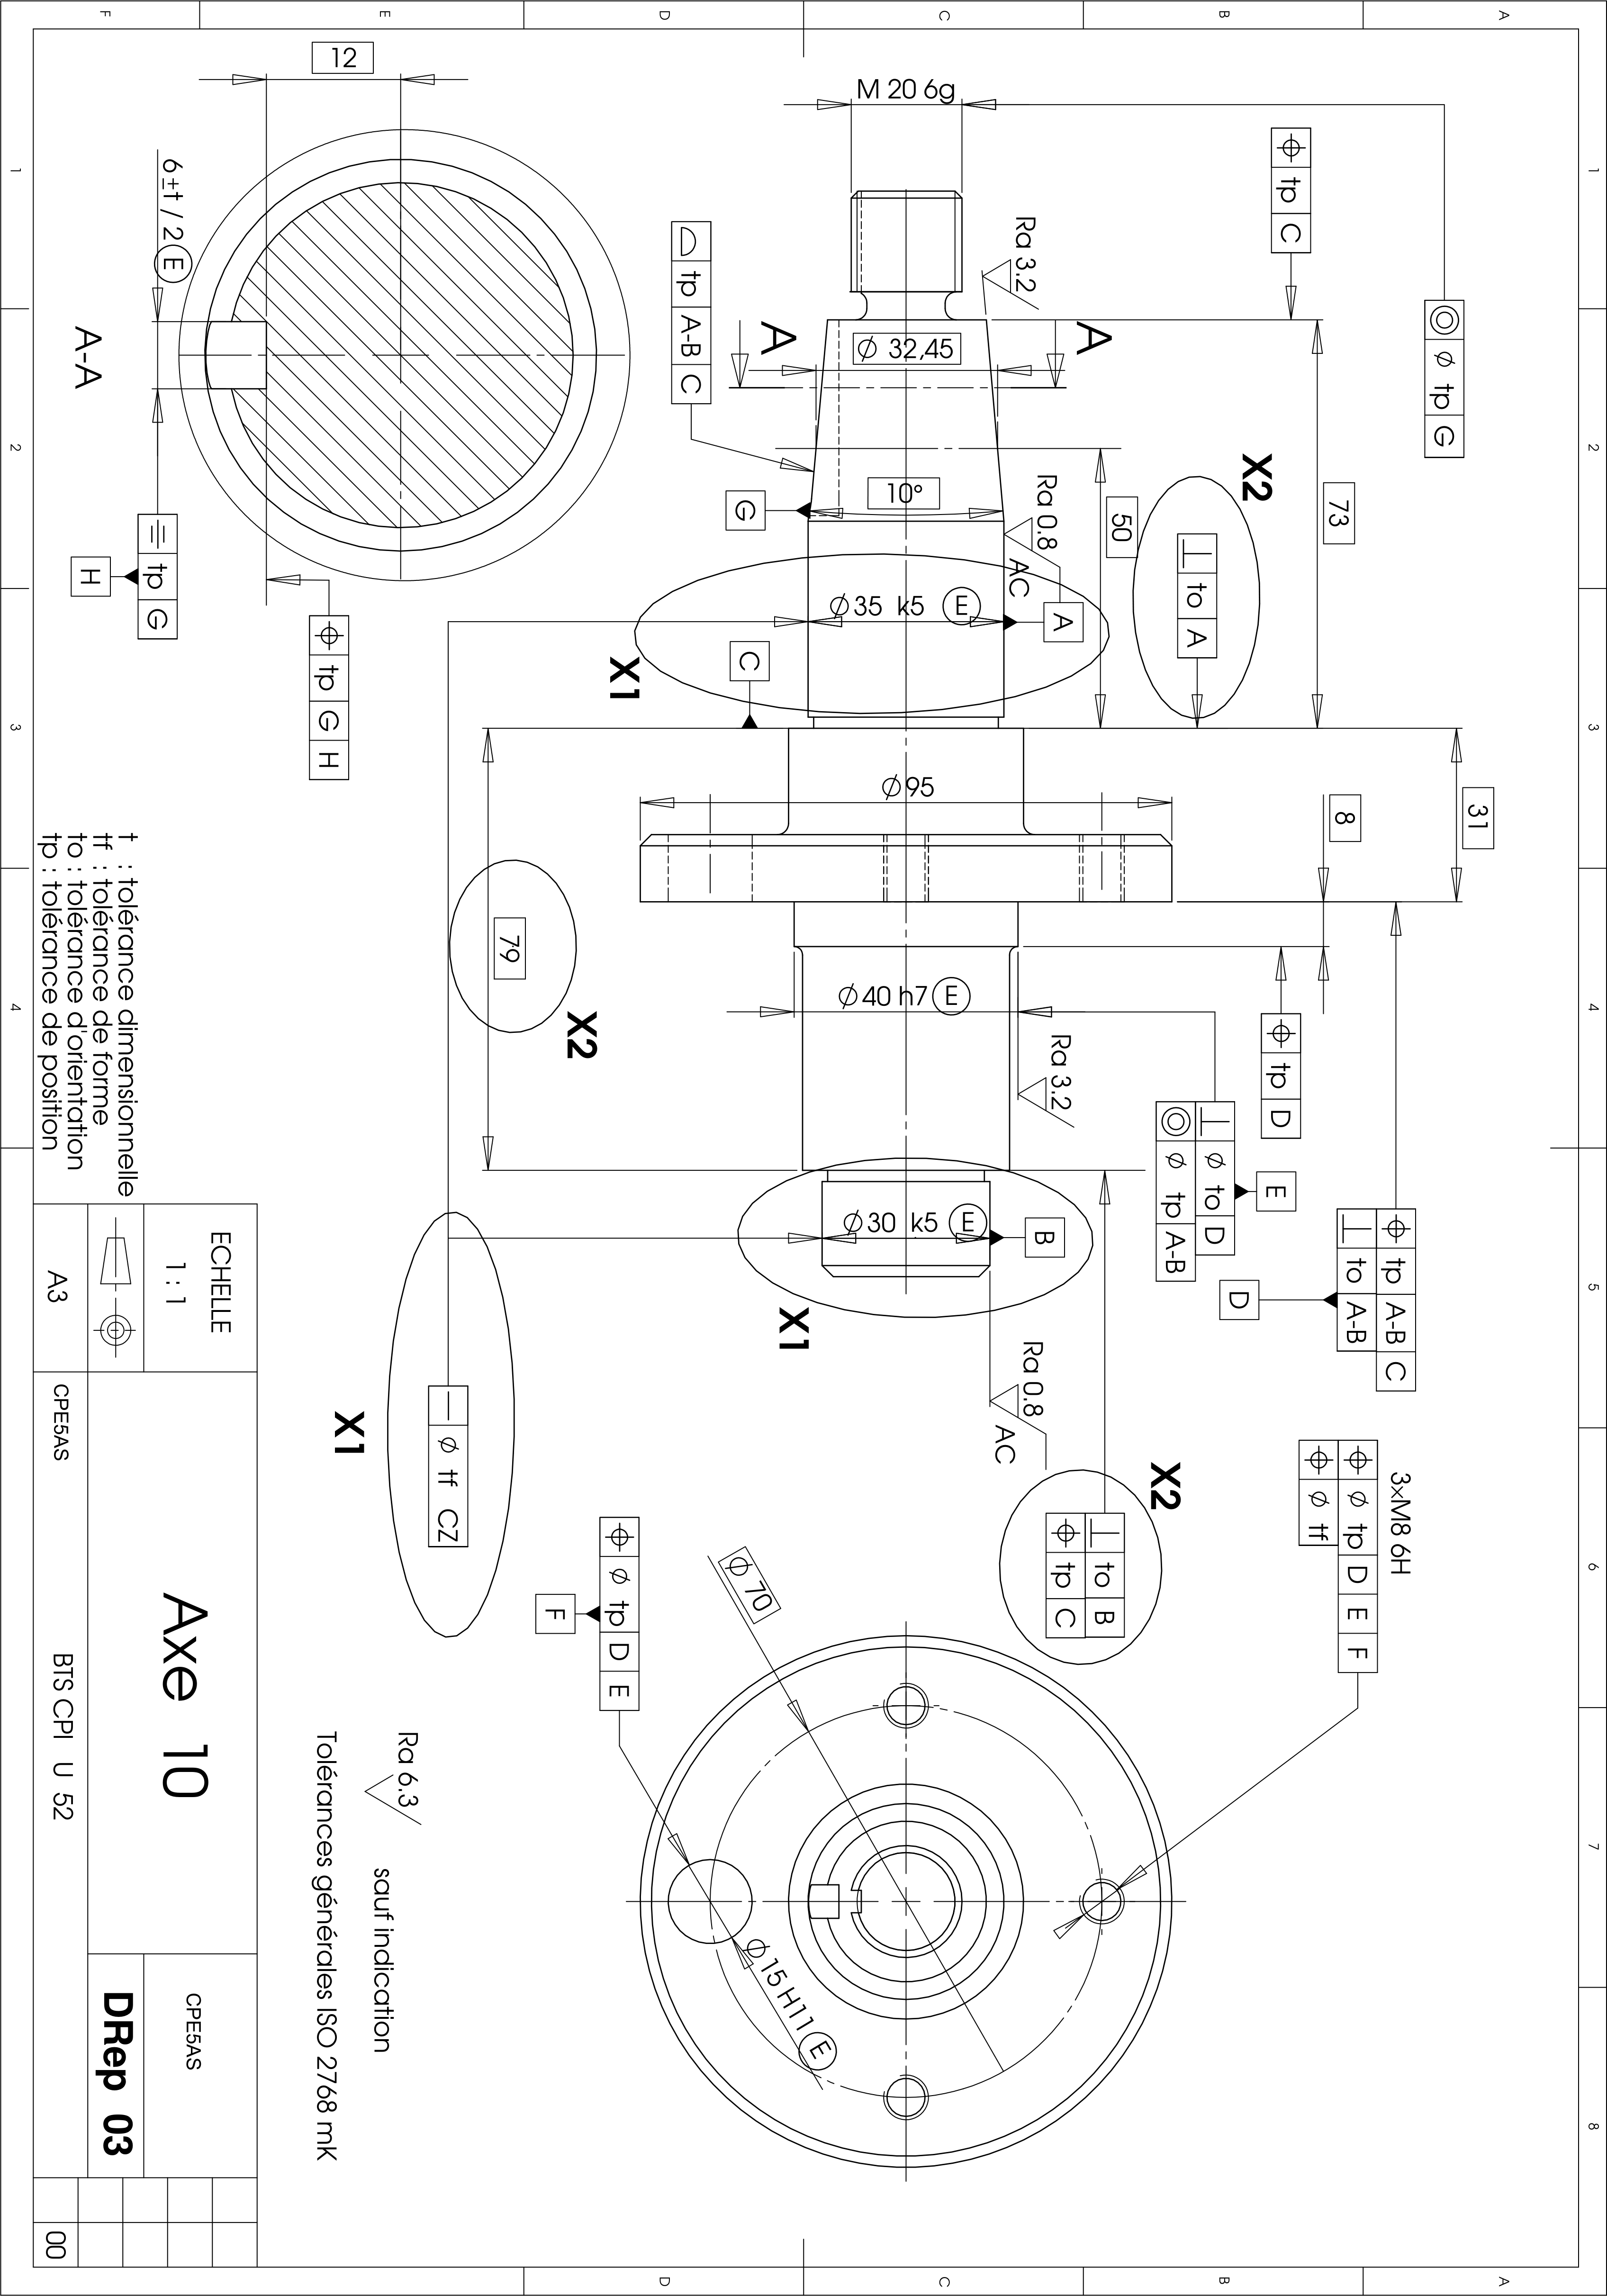
\includegraphics[width=\linewidth]{74_04}

\ifprof
\else
\begin{flushright}
\footnotesize{Corrigé  voir \ref{A5:05:74}.}
\end{flushright}%
\fi 